% last updated in April 2002 by Antje Endemann
% Based on CVPR 07 and LNCS, with modifications by DAF, AZ and elle, 2008 and AA, 2010, and CC, 2011; TT, 2014; AAS, 2016

\documentclass{llncs}
\usepackage{graphicx}
\usepackage{amsmath,amssymb} % define this before the line numbering.
\usepackage{ruler}
\usepackage[dvipsnames]{xcolor}
\usepackage{subcaption}
\captionsetup{compatibility=false}
\usepackage{xcolor}
\usepackage[width=122mm,left=12mm,paperwidth=146mm,height=193mm,top=12mm,paperheight=217mm]{geometry}
\usepackage{multirow}
\usepackage{algorithm}
\usepackage[]{algpseudocode}
\newcommand{\jason}[1]{\textcolor{orange}{\textbf{JASON: #1}}}
\newcommand{\madan}[1]{\textcolor{red}{#1}}

\begin{document}
% \renewcommand\thelinenumber{\color[rgb]{0.2,0.5,0.8}\normalfont\sffamily\scriptsize\arabic{linenumber}\color[rgb]{0,0,0}}
% \renewcommand\makeLineNumber {\hss\thelinenumber\ \hspace{6mm} \rlap{\hskip\textwidth\ \hspace{6.5mm}\thelinenumber}}
% \linenumbers
\pagestyle{headings}
\mainmatter
\def\ECCV18SubNumber{1816}  % Insert your submission number here

\title{TARP: Tensorflow-based Activity Recognition Platform} % Replace with your title

\titlerunning{TARP: Tensorflow-based Activity Recognition Platform}

\authorrunning{Eric Hofesmann, Madan Ravi Ganesh, \and Jason J. Corso}

\author{Eric Hofesmann, Madan Ravi Ganesh, \and Jason J. Corso}
\institute{University of Michigan}
\newcommand{\acro}{TARP}
\newcommand{\model}{\textbf{Model submodule}}
\newcommand{\checkpoint}{\textbf{Checkpoint submodule}}
\newcommand{\metrics}{\textbf{Metrics submodule}}
\newcommand{\data}{\textbf{Input Data Block}}
\newcommand{\exec}{\textbf{Execution Block}}

\maketitle

\begin{abstract}
Action recognition is a widely known and popular task that is essential to build up knowledge for video understanding.
The absence of an easy-to-use platform containing state-of-the-art (SOTA) models presents an issue for the community.
Given that individual research code is not written with an end user in mind and in certain cases code is not released, even for published articles, the importance of a common unified platform capable of delivering results while removing the burden of developing an entire system is further underlined.
To try and overcome these issues, we develop a tensorflow-based unified platform to abstract away unnecessary overheads in terms of an end-to-end pipeline setup in order to allow the end user to quickly and easily prototype action recognition models.
With the use of a consistent coding style across different models and seamless data flow between various submodules, the platform lends itself to the quick generation of results on a wide range of SOTA methods across a variety of datasets.
All of these features are made possible through the use of a fully pre-defined training and testing pipeline built on top of a small but powerful set of modular functions that handle asynchronous data loading, model initializations, metric calculations, saving and loading of checkpoints, and logging of results.
The platform is geared towards easily creating models, with the minimum requirement being the definition of a network architecture and preprocessing steps from a large custom selection of layers and preprocessing functions.
\acro~currently houses four SOTA activity recognition models which include, I3D, C3D, ResNet50+LSTM and TSN.
The recognition performed achieved by these models are, $XX\%$ for ResNet50+LSTM and $YY\%$ for C3D on XXXXX while I3D and TSN achieve $ZZ\%$ and $QQ\%$ on YYYYY respectively.

\keywords{tensorflow, activity recognition, framework, state-of-the-art models, C3D, I3D, Temporal Segment Networks, ConvNet+LSTM}
\end{abstract}

\section{Introduction}
\label{sec:intro}

The research community is focused on exploring concepts at the frontiers on science and help solve problems that bog our development down.
An important part of research is the analysis of currently proposed theories and further improving upon them. 
This necessitates the use and re-use of models and theories that are currently state-of-the-art. 
However, given the strong emphasis on concepts and modelling, coding is relegated to a lower priority.
Thus, there isn't a universal standard guideline for coding practice and this leads to strong variations from place to place and even between communities within a university.
Further, not all the components that are needed to re-create the results published are provided to the research community, which takes away from valuable time spent on research and instead is used to replicate the published results through common knowledge, details published in the paper and a little guesswork.
In this paper, we propose to solve this problem in the context of action recognition in the field of computer vision.

There has been a recent positive trend towards open sourcing code, in the computer vision community.
However, even when the same language is used to develop software, custom coding practices make it extremely difficult to quickly assimilate and integrate code.
When custom coding styles are combined with the vast array of languages available, e.g., tensorflow~\cite{}, pytoch~\cite{}, caffe~\cite{} in deep learning, it adds to the complexity since key words in languages tend to vary in meaning and this necessitates an extremely deep understanding of each and every language.
Subtle differences, such as, the keyword ``\texttt{\textcolor{ForestGreen}{dropout ratio}}'' can mean the ratio of nodes to drop or keep, can have massive impacts on the final results.
When put into the context of feature exatraction, each deep learning language has a model zoo to access a number of staples. However, we aren't aware of such a model zoo for a task like activity recognition. 
Given the popularity of activity recognition, as a precursor to video understanding, and the prevalence of deep learning it is surprising.

In order to avoid the complication of parsing code between different language and the complications that can arise from doing so, we use a single language, tensorflow, for our platform.
We further supplement it with a suite of state-of-the-art activity recognition models.
The existences of SOTA models removes the necessity of replication and the end user can focus their time on implementing deep learning models and conduct research.
For this purpose, we provide \acro~which is a platform that allows the user to solely focus on the creation or fine-tuning of models by abstracting away unnecessary peripheral details like data input, computing metrics, and extracting features.

The main contributions of the platform are:
\begin{itemize}
\item Extract features from SOTA activity recognition models.
\item Quickly generate results across a combination of a variety of dataset and ANN models.
\item Single node multi-GPU expansion support to train and fine-tune models.
\item A custom input pipeline that condenses the loading and processing of videos into a set of flexible and easy-to-use options for the user.
\item The ability to convert model weights, stored in our custom Numpy dictionary format, to alternative formats used in other deep learning languages..
\item A vast array of customized options for neural network layer definitions and preprocessing functions.
\end{itemize}

Within this report, we use the following formatting techinques,
\begin{itemize}
\item \textcolor{red}{loss} - To denote functions
\item \textcolor{blue}{file.npy} - To denote different file names
\item \texttt{\textcolor{ForestGreen}{loss\_type}} - To denote keywords in the code
\item \textbf{Model block} - To denote Blocks, submodules and any higher level construct
\end{itemize}

\begin{figure}[b!]
\centering
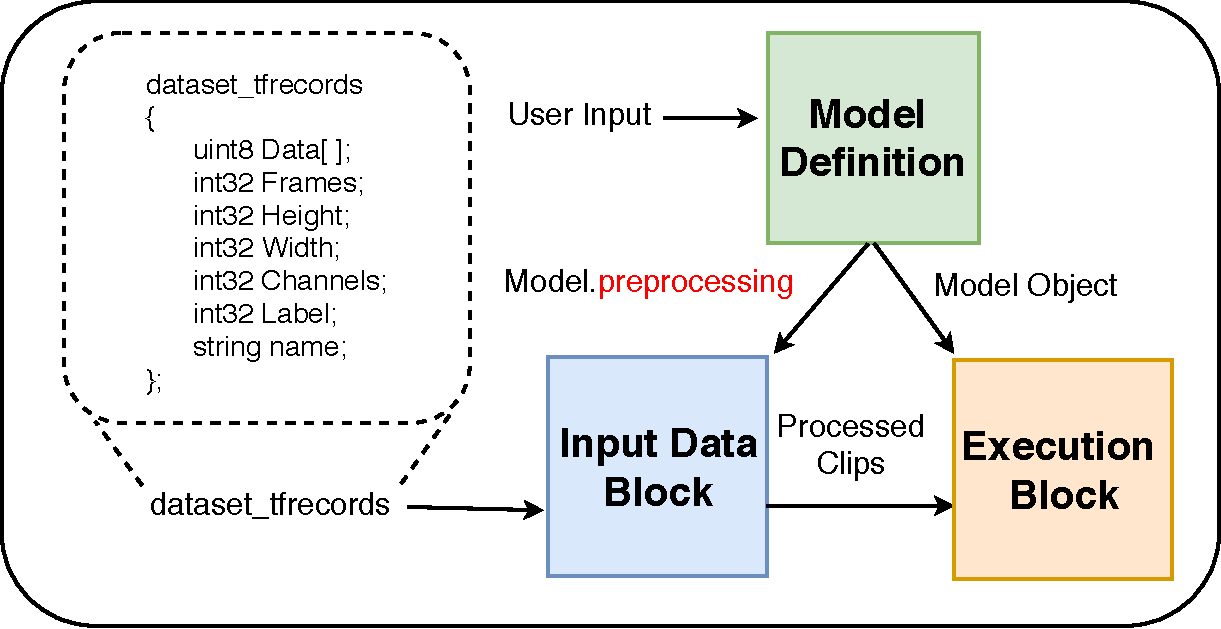
\includegraphics[width=0.8\textwidth]{images/overview.pdf}
\caption{Illustration of the three main components of \acro}
\label{fig:overview}
\end{figure}


\section{Overview of \acro}
\label{sec:overview}

\acro~is comprised of three main components, 1) the \textbf{Input Data Block}, 2) \textbf{Model Definition Block} and 3) the \textbf{Execution Block}, as shown in Fig.~\ref{fig:overview}.
The pipeline contained within the \textbf{Input Data Block} can be divided into three simple stages,
\begin{enumerate}
\item Read video data from disk
\item Extract the desired number of clips from a given video
\item Preprocess the frames of clips using a selected model's preprocessing strategy.
\end{enumerate}
On the other hand, the \textbf{Execution Block} houses all of the code required to setup, train, test as well as log the outputs of a chosen model.
This includes defining the layers that comprise the model, training the model up to a predetermined number of epochs, saving parameter values of a model are regular intervals and finally testing the performance of the trained model over a variety of recognition metrics.
The following sections provide an in depth discussion of the setup and structure of various components that make up the \textbf{Input Data} and \textbf{Execution Blocks}.

\section{Input Data Block}
\label{sec:ipblock}
Included in the \textbf{Input Data Block} are all of the steps required to load a video and process it into the proper format.
Fig.~\ref{fig:ip_block} shows the structure and flow of data as it passes through the \textbf{Input Data Block}.
The three stages of the \textbf{Input Data Block}, reading video data, extracting clips, and preprocessing clips, are detailed below.

\begin{figure}[t!]
\centering
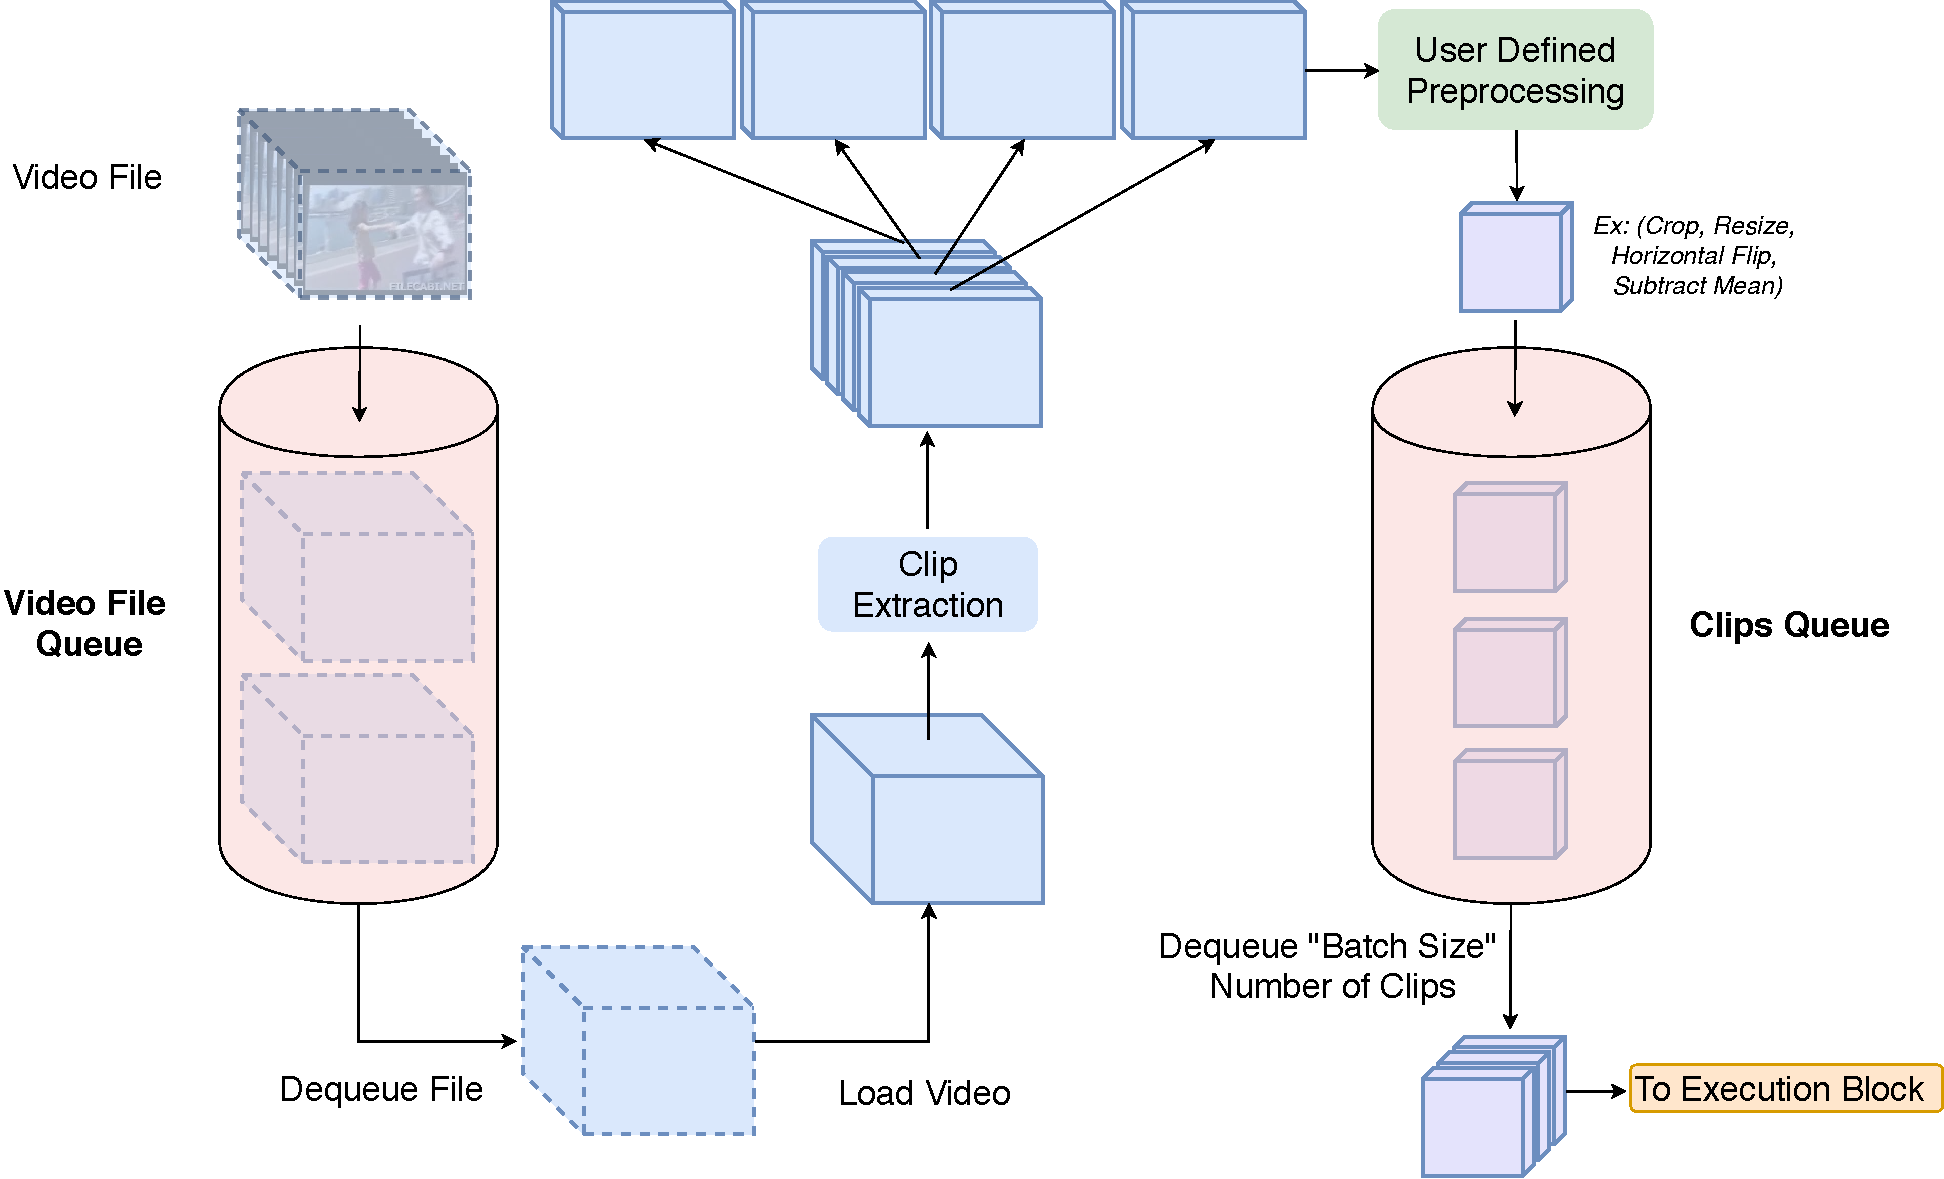
\includegraphics[width=1.0\columnwidth]{images/ip_pipeline.pdf}
\caption{This figure depicts the data flow from loading video files to passing a processed batch of clips into the specified model.
The input pipeline is structured around two separate queues, one queue for storing file names of all tfrecords in the specified dataset and another queue for storing processed clips waiting to be passed to the model.
During runtime, the \texttt{\textcolor{ForestGreen}{video\_file\_queue}} gets filled with all available tfrecords filenames in a given dataset, which then get dequeued one by one.
The video corresponding to a dequeued file name gets loaded into the system and broken down into clips as described in Sec.~\ref{sec:extractclips} and Fig.~\ref{fig:extract_clips}.
Each clip then gets individually preprocessed according to a set of user defined steps as described in Sec.~\ref{sec:modeldefblock}.
The processed queues then get loaded into the \texttt{\textcolor{ForestGreen}{clips\_queue}} so that exactly one \texttt{\textcolor{ForestGreen}{batch\_size}} of clips is available to be loaded into the model.}
\label{fig:ip_block}
\end{figure}


\subsection{Read video data}
\label{sec:readdata}
In \acro, video data is stored in the form of tfrecords files to allow the entire \textbf{Input Data Block} to be constructed into the tensorflow graph for efficient parallel data loading.
These files can be generated using provided scripts and examples, assuming that the original video datasets have been acquired.
The contents of these files include the video height, width, channels, number of frames, BGR data, name of the video file, and the label of the action class related to the video.
Video data is stored in BGR format due to the use of OpenCV for converting the original video files to python arrays.
The first step of the input pipeline after reading in the tfrecords data is to convert the video to RGB.

Reading tfrecords files is accomplished through the use of a \texttt{\textcolor{ForestGreen}{tfrecord\_file\_queue}} which stores the names of all tfrecords in the given dataset directory.
After a file name has been extracted form this queue, the corresponding video will then be broken down into clips and preprocessed.
To allow for the loading of multiple clips from each video, a \texttt{\textcolor{ForestGreen}{clips\_queue}} is added to the pipeline to store individual clips.

Note: When loading the dataset HMDB51, videos are stored in a 30 frames-per-second (fps) format while most models require 25 fps. A function, \textcolor{red}{\_reduce\_fps} is used to remove every sixth frame from HMDB51 videos in order to reduce the fps.


\subsection{Extract clips}
\label{sec:extractclips}
Certain models, for example C3D~\ref{}, require their inputs to be in the form of multiple clips extracted from a single video.
Fig.~\ref{fig:extract_clips} details the various arguments that are available to break down a video into clips.
These methods shown are able to be used in conjunction with one another to give the user the flexibility needed to extract clips with different dimensions.
All of this can be done through the use of only a handful of arguments including \texttt{\textcolor{ForestGreen}{clip\_length}}, \texttt{\textcolor{ForestGreen}{num\_clips}}, \texttt{\textcolor{ForestGreen}{clip\_offset}}, and \texttt{\textcolor{ForestGreen}{clip\_stride}}
By default, the clip extraction algorithm is set to process and entire video at a time and only extract clips if the required arguments have been specified.
In addition to the options shown in Fig.~\ref{fig:extract_clips}, \acro~also provides options for random selection of clips.

\begin{figure}[b!]
\centering
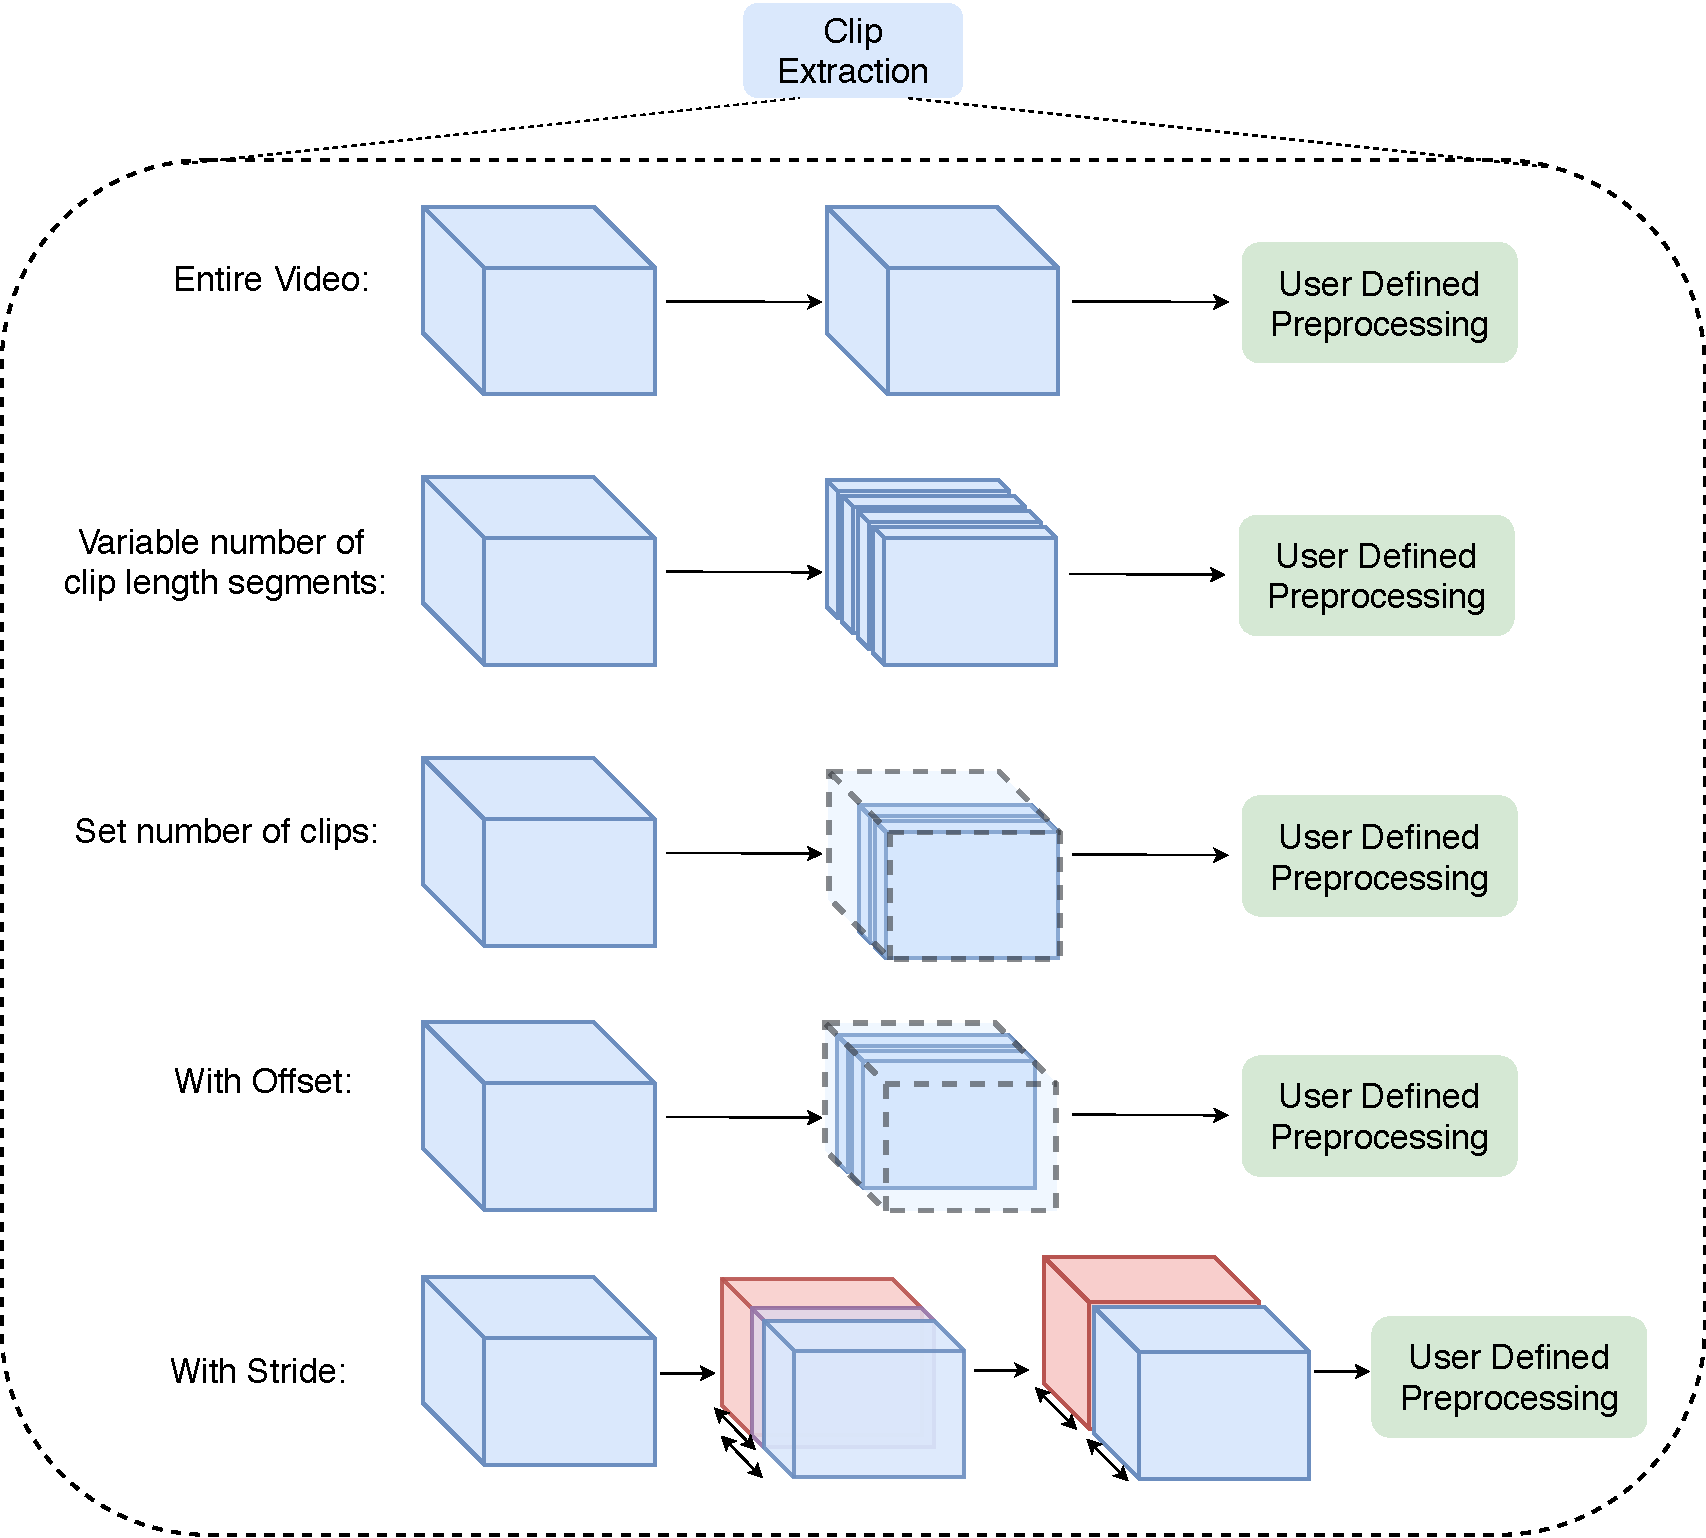
\includegraphics[width=0.8\columnwidth]{images/extract_clips.pdf}
\caption{This figure shows the varying ways that a video can be broken into clips.
By default the entire video is passed directly on to the user defined preprocessing without any modifications.
A variable number of clips can be extracted from a video if only the \texttt{\textcolor{ForestGreen}{clip\_length}} parameter is given.
Due to this variablity, the implementation of the \texttt{\textcolor{ForestGreen}{clips\_queue}y} is critical.
Alternatively, a set number of clips of a certain length can be extracted from every video using the \texttt{\textcolor{ForestGreen}{num\_clips}} parameter.
If a video does not contain enough frames to extract the requested number of clips, the video will be looped until the necessary frame count is reached.
There also exists an \texttt{\textcolor{ForestGreen}{offset}} parameter which can be set to randomly modify where from the beginning of the video the function begins to extract clips. 
The \texttt{\textcolor{ForestGreen}{stride}}  parameter can be used to set a number of frames that will be common between sequential clips.
This \texttt{\textcolor{ForestGreen}{stride}} parameter can be set to a negative value to skip a set number of frames between sequential clips.
}
\label{fig:extract_clips}
\end{figure}


The desired preprocessing file for a model can be defined within the \textbf{Model Submodule} and will be used automatically in the \textbf{Input Data Block} after a video has been broken down into clips.
Preprocessed clips can significantly vary in shape when compared to the input video.
Any change in frame height, width, or number of frames is allowed as long as clips are not broken down further.
The \texttt{\textcolor{ForestGreen}{clips\_queue}} is designed to be compatible with any dimensionality of clips, as long as all clips that are being stored have the same dimensionality.
More specifically, processed clips must be of the shape [\texttt{\textcolor{ForestGreen}{input\_dimensions}}, \texttt{\textcolor{ForestGreen}{size}}, \texttt{\textcolor{ForestGreen}{size}}, \texttt{\textcolor{ForestGreen}{sequence\_length}}] for the entirety of a training or testing session.

Note: Due to the nature of tensorflow enqueue operations, errors that occur within an enqueue operation do not properly throw an error.
The enqueue is simply canceled and an error will occur when the dequeue attempts to access an empty queue.
This effect occurs within the \texttt{\textcolor{ForestGreen}{clips\_q}} if an error occurs in the user defined preprocessing submodule.
In order to allow proper debugging of the preprocessing submodule, the argument \texttt{\textcolor{ForestGreen}{preprocDebugging}} is available to bypass the \texttt{\textcolor{ForestGreen}{clips\_q}} and see any error tracebacks.
Since the queue used to store clips is removed, the requirement is set that \texttt{\textcolor{ForestGreen}{batch\_size}} must equal \texttt{\textcolor{ForestGreen}{num\_clips}} while debugging.



\section{Model Definition Block}
\label{sec:modeldefblock}

\begin{figure}[b!]
\centering
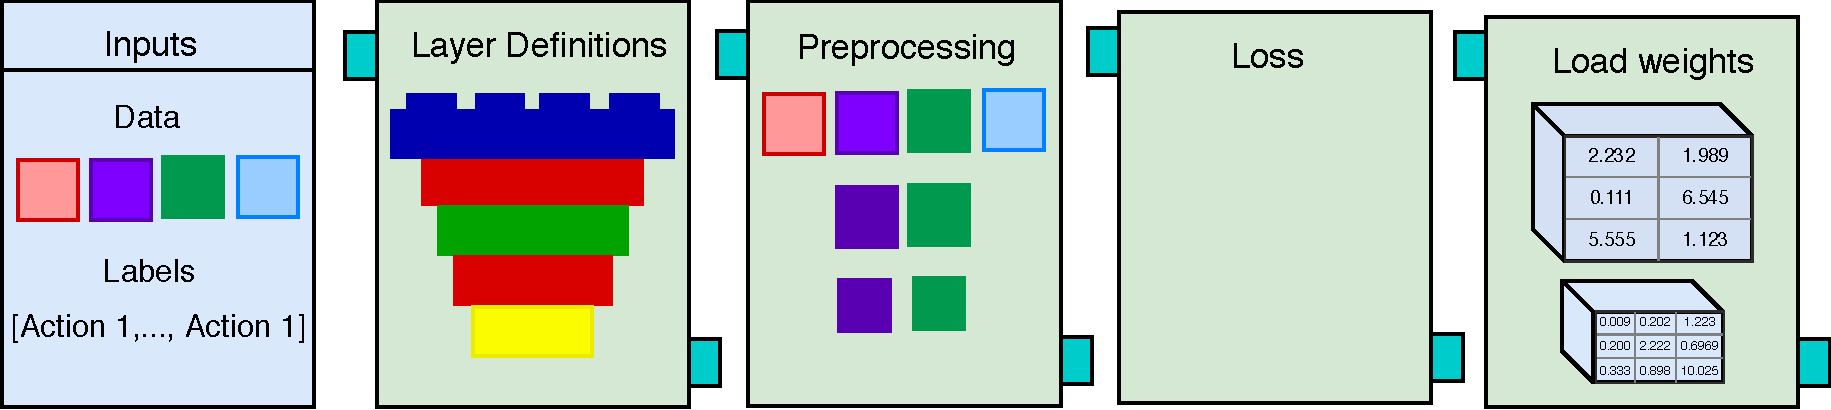
\includegraphics[width=\columnwidth]{images/model_submodule.pdf}
\caption{}
\label{fig:model_submodule}
\end{figure}


\subsection{Preprocessing}
The class definition of a model within \acro~can be divided into four main components as shown in Fig.~\ref{fig:model_submodule}.
Preprocessing is the first module in the \model that gets used within \data.
Activity recognition models employ a number of various preprocessing methods on a frame or clip-based level often used for data augmentation.
These can include frame-wise cropping, flipping, and resizing, or clip-wise cropping, flipping, temporal offsets, resampling, looping, and more.
In keeping with the modular design paradigm, we use individual functions to define each variant of the preprocessing pipeline.
By keeping each variant within its own file, marked with the suffix ``\textcolor{blue}{\_preprocessing.py}'', we increase their reusability and ensure debugging them is easy.
Within the class definition of a model, multiple preprocessing pipelines can be included using a simple \textit{if-else} construct.
The expected final product from any preprocessing function is the complete preprocessed input data that needs to be passed into a network's input layer.




\subsection{Model Architecture}
The definition of a model's input layer and the subsequent layers that make up the model's network architecture should be present within the \textcolor{red}{inference} function.
The layers used must strictly be called from within the set of definitions provided within the \textcolor{blue}{layer\_utils} file.
This ensures that layer definitions are not specific to any network and become available to all models defined within \acro.
Further, it is essential that the inference function returns the outcome of any and all desired layers from within the defined network.
Any accompanying functions to help quickly and/or recursively define a network can be added outisde of the inference function.


\subsection{Loss and Loading Weights}
As a minor deviation from standard practices, we attach the definition of a loss to the model definition instead of the main training file.
We do this to avoid cluttering and increasing the complexity of the main training file.
Thus, a prime requirement within any model definition is the implementation of a loss function, with the expected return from this function being the final loss value.
To add further flexibility in using multiple losses with a single model, the basic loss function can alternatively be overloaded to call different losses using the internally defined \texttt{\textcolor{ForestGreen}{loss\_type}} keyword.

The final and optional component of any model definition within \acro~is the definition of the \textcolor{red}{load\_default\_weights} function.
This function is defined to ensure that a predetermined set of weights can be loaded into a network's layers.
The explicit rules required to define the layer names and ensure their respective weights can be assigned are provided in Section~\ref{sec:checkpoint}.
The final values returned by this function are the parameter weights loaded from an external file.

\subsection{Automatic Template Generation}
Given that the focus of \acro~is to help the end-user quickly define and integrate a model to the framework, we provide a template file named \textcolor{blue}{models\_template.py} which provides the outline for the user to quickly fill out the inference, preprocessing, loss and load weights functions.
A separate file named \textcolor{blue}{models\_preprocessing\_template.py} provides an outline of the necessary function to defining the preprocessing pipeline.
Once a model has been completely defined, it is automatically imported into the framework through a recursive call strategy.
To quickly track and log a model class variable an inbuilt dictionary named \texttt{\textcolor{ForestGreen}{track\_variables}} is available.
Adding any pre-defined variable name and graph title allows the logging of the desired variable on tensorboard.

Note: 1) Any model defined must be placed within the models folder under a directory with the same name as that of the model,
2) The actual model file must be named with a suffix ``\textcolor{blue}{\_model}''.
2) No explicit model class attributes can be added to a specific model. Instead, they must be added to the \textcolor{blue}{model\_abstract.py} file and made available to any and all model definitions within \acro.

The models that come standard with \acro~include the state-of-the-art activity recognition architectures I3D~\cite{}, C3D~\cite{}, ResNet50~\cite{}, and TSN~\cite{}.




\section{Execution Block}
\label{sec:execblock}
The execution block form the largest component of the entire platform. Its code can be broken down into parts that are used during two alternate phases, training and testing.
Fig.~\ref{fig:exec_block} illustrates this concept and highlights the submodules used within each phase.
An algorithmic overview of each phase, followed by a detailed description of the various submodules used within them are provided in the following sections.

\begin{figure}[t!]
\centering
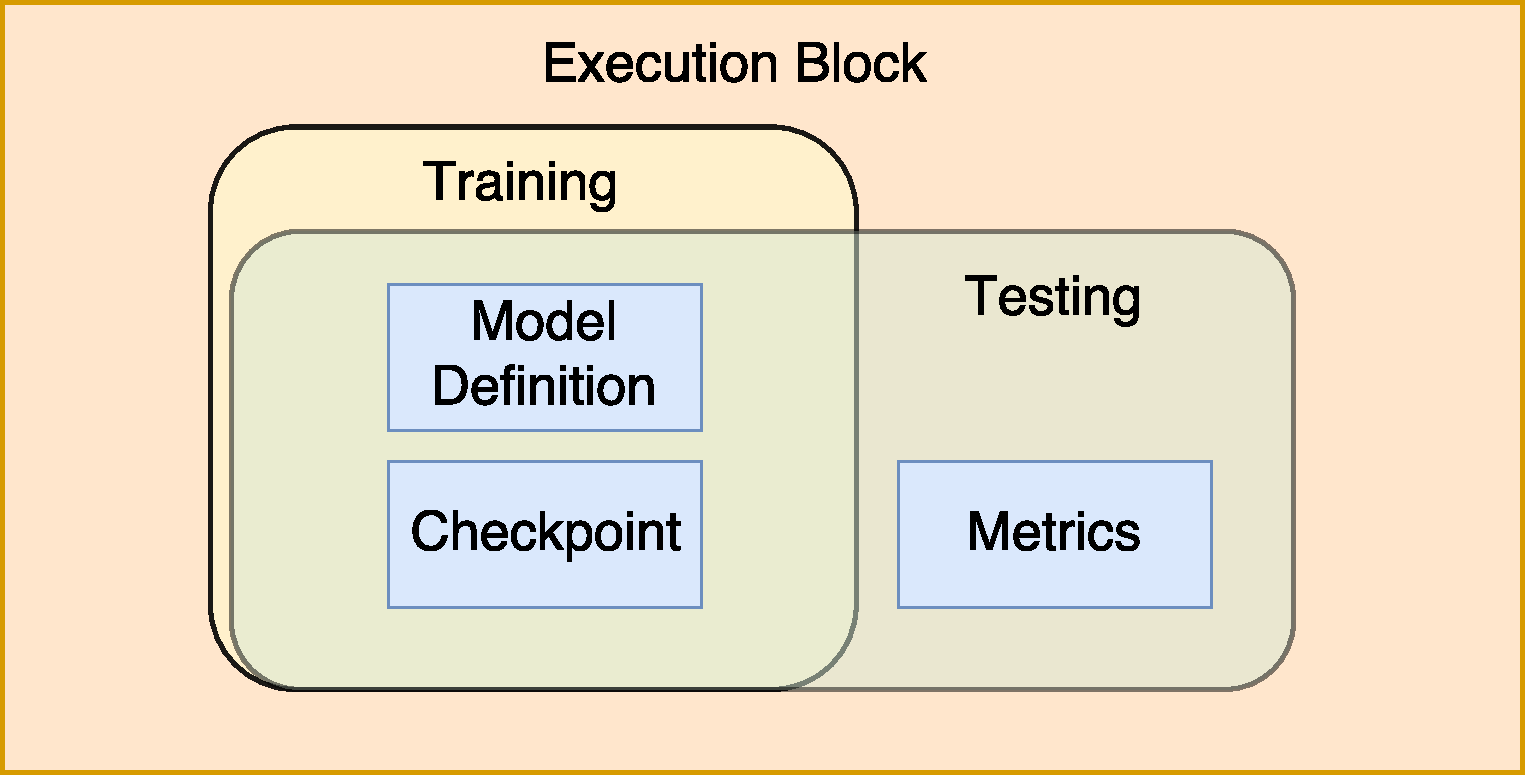
\includegraphics[width=0.8\columnwidth]{images/exec_block.pdf}
\caption{Training and Testing functions are the two major phases within the execution block. Model definitions and checkpoint-based functions are part of both training and testing functions while metrics are calculated after models are tested.}
\label{fig:exec_block}
\end{figure}

\subsection{Training: Flow of processes}
\label{sec:training}
Training, within the context of the execution block, follows the process flow outlined in Alg.~\ref{}.
The beginning of every training phase is associated with the selection and set up of a model.
Basic model parameters such as input/output data dimensions, batch normalization, dropout rate, and etc. are passed into the \model~for this purpose.

Once the model has been set up, the next step is to ensure that the parameter weights for the chosen model are retrieved.
If the model has been pre-trained using \acro~and the user desires to further fine-tune the model, then the model parameter's weights from the latest checkpoint will be restored.
By default, the standard pre-trained weights are loaded into the model.
Alternatively, a random initialization option, for users to train a model from scratch is also provided.
As a backup when a specified checkpoint is unavailable, the system defaults to the random intialization option, with an additional warning provided to the user about the setup being used.

After the preparation of the model is complete, data tensors are retrieved from the \data~ and interfaced to the model.
The main data retuned from \data~are the video frames, their corresponding labels and video names.
With the availability of the model and data, the next step is to create a copy of the model on each of the selected number of GPUs within a compute node.
Within each GPU, the inference function of \model~is used to generate a copy of the layer definitions.
Here, the variable names are re-used to ensure that the same copy of weights are associated throughout all the GPUs.
\acro~only supports the extension of a model within a compute node of a cluster.
Currently, it cannot be distrbute a model across mutiple nodes or split a model across multiple GPUs within a node.

From each of the model copies, we retrieve a desired layer's output.
Given that the most common approach to training a network is through the use of logits returned from the final layer, we use the variable logits, associated with the last layer, to obtain a loss value.
Finally, the loss and gradients, computed from the loss, across all the model copies are accumulated into the loss\_array and gradients\_array respectively.
The contribution of each model copy is weighted equally and the final gradient used to update the weights of the model is obtained by taking the average of value stored in the gradients\_array.
The is the final stage in the definition of the tensorflow graph required for training.

\begin{algorithmic}[H]
\Procedure{Training}{}
\State \textbf{Model\_definition}.\textcolor{red}{setup}(model\_params)
\State \textbf{Checkpoint}.\textcolor{red}{load\_param\_weights}(default or specific file)
\State Data, Labels = \textbf{DIB}.\textcolor{red}{load\_data}(expt\_params)
\\
\For{each GPU within given node}
\State \textbf{Model\_definition}.\textcolor{red}{inference}(Data, model\_params)
\State tower\_loss = \textbf{Model\_definition}.\textcolor{red}{loss}(Labels, returned\_logits)
\State tower\_gradients = gradients(tower\_loss)
\State loss\_array.store(tower\_loss)
\State gradients\_array.store(tower\_gradients)
\EndFor
\\
\State grad = average\_gradients(gradients\_array)
\State train\_op = apply\_gradients(grad)
\\
\While{no\_videos\_loaded \textless~(total\_epochs $\times$ videos\_in\_dataset)}
\State \textbf{Checkpoint}.\textcolor{red}{save}() @ regular intervals
\State sess.run(train\_op)
\State update(no\_videos\_loaded)
\EndWhile
\EndProcedure
\end{algorithmic}

After the tensorflow graph for training has been defined, the next step is to execute the graph.
Usually, models are trained for a typical number of epochs, iterations over the entire dataset.
Within each epoch, based on a set frequency of iterations, we save the model parameter's weights using \checkpoint.save().
The main operation that gets executed within each iteration is the training operation that links the calculation of losses, gradients and their application.
It is important to note that during the setup of the experiment, \acro~ offers adaptive learning rate control which steps down the learning rate when the loss plateaus.
The repeated application of train\_op forms the most crucial and final step in the training process flow.



\subsection{Testing: Flow of processes}
\label{sec:testing}

Testing begins similarly to training in that a specified model gets defined and initialized according to given parameters.
The model parameters during testing are identical to those used to instantiate a model during training.
Other input arguments that do exist when testing that are not used during training include \texttt{\textcolor{ForestGreen}{metrics\_method}}, \texttt{\textcolor{ForestGreen}{return\_layer}}, and \texttt{\textcolor{ForestGreen}{avg\_clips}}.

After a model object has been instantiated, the model weights are loaded.
The option exists to either load the weights from the default weight file specified within the \textbf{Model Submodule} or to initialize the model to random weights if that is desired.
Most commly, however, the \textbf{Checkpoint Submodule} is used to load the checkpoints of a model that has been trained from scratch or fine-tuned.

Once the model weights are accessible, the dataset will be loaded into the system following the process described in the \textbf{Data Input Block} in Sec.~\ref{sec:ippipeline}.
Videos are not shuffled when being loaded for testing so that all testing instances are directly comparable.
The shape of this input data is set to allow for any number of different videos or multiple clips of a single video to be loaded for testing.
More specifically, the \texttt{\textcolor{ForestGreen}{batch\_size}} of input data can be used to load multiple clips of a single video in order to determine a consensus across these clips which will act as the prediction for the entire video as explained in C3D~\cite{}.
In addition, this \texttt{\textcolor{ForestGreen}{batch\_size}} parameter can also load multiple videos simultaneously if videos are broken into a number of clips which is smaller than the batch.
No models currently use this multiple video functionality for testing, videos are loaded one at a time for testing and only batched for training, but it is available if needed in the future.

Before the data can be loaded into the model, the model must first be copied onto the GPU.
While only a single GPU is used for testing, a GPU list can still be given to \acro~to determine which GPU the testing instance will be assigned to.
If the list contains more than one GPU device id, the first element in that list will be used.
The process of copying the model to the GPU is based around the \textbf{Model\_definition.}\textcolor{red}{inference} call which will return the output of the layer specified in the \texttt{\textcolor{ForestGreen}{return\_layer}} argument.
By default, the layer that will be returned by \textbf{Model\_definition.}\textcolor{red}{inference} are of the shape [\texttt{\textcolor{ForestGreen}{batch\_size}}, \texttt{\textcolor{ForestGreen}{sequence\_length}}, \texttt{\textcolor{ForestGreen}{output\_dimensions}}] and then converted to action class predictions using the softmax function.
This shape is only required when the \texttt{\textcolor{ForestGreen}{logits}} layer is returned from the \textcolor{red}{inference} call and the application of softmax is dependent on the \texttt{\textcolor{ForestGreen}{useSoftmax}} argument.
With the model output acquired, the final stepis of preparation for testing is to set up the output directory structure, the \textbf{Metrics Submodule} detailed in Sec.~\ref{sec:metrics}, and to load weights into the model as described in the \textbf{Checkpoints Submodule} in Sec.~\ref{sec:checkpoint}.

The testing block iterates through the \texttt{\textcolor{ForestGreen}{num\_vids}} specified which generally includes an entire testing split of a dataset.
Within this block, the tensorflow session is run to extract the model's \texttt{\textcolor{ForestGreen}{output\_predictions}}, ground truth \texttt{\textcolor{ForestGreen}{labels}}, and all video \texttt{\textcolor{ForestGreen}{names}} in this batch.
If the \texttt{\textcolor{ForestGreen}{avg\_clips}} argument has been specified, then the \texttt{\textcolor{ForestGreen}{output\_predictions}} are averaged over their first dimension which is \texttt{\textcolor{ForestGreen}{batch\_size}} or in this case, the number of clips loaded for this testing iteration.
A tracker counts the number of videos that have been loaded using the video \texttt{\textcolor{ForestGreen}{names}} output.
The \texttt{\textcolor{ForestGreen}{output\_predictions}} and ground truth \texttt{\textcolor{ForestGreen}{labels}} are then fed into the \textbf{Metrics Submodule} for logging and storing.
Finally, the thread coordinator for the input queues is stopped and the all predictions from the \textbf{Metrics Submodule} are saved as a numpy format.

\begin{algorithmic}[H]
\Procedure{Testing}{}
\State \textbf{Model\_definition}.\textcolor{red}{setup}(model\_params)
\State \textbf{Checkpoint}.\textcolor{red}{load\_param\_weights}(default or specific file)
\State Data, Labels = \textbf{DIB}.\textcolor{red}{load\_data}(expt\_params)
\\
\For{one GPU}
\State \textbf{Model\_definition}.\textcolor{red}{inference}(Data, model\_params, return\_layer)
\If{use\_softmax}
\State logits = softmax(logits)
\EndIf
\EndFor
\\
\State \textbf{Metrics}()
\\
\While{num\_videos\_loaded \textless~videos\_in\_dataset}
\State output\_predictions = sess.run(logits)
\If{average\_over\_clips}
\State mean(output\_predictions, 0)
\EndIf
\State \textbf{Metrics.}\textcolor{red}{log\_prediction}(output\_predictions)
\State update(num\_videos\_loaded)
\EndWhile
\EndProcedure
\end{algorithmic}


\subsection{Checkpoint Submodule}
\label{sec:checkpoint}
The checkpoint submodule contains utility functions that handle all the essential functions w.r.t. checkpoints.
Checkpoints themselves are stored in a custom format as shown in Fig.~\ref{}.
This format readily lends itself to a recursive access strategy while offering easy conversion capabilities from its native numpy format to ``\textcolor{blue}{.ckpt}'',``\textcolor{blue}{.caffemodel}'' and other formats.
Among the variety of operations that can be performed on and using checkpoints, there are two broad categories, Load/Save and Tensor handling.

\paragraph{Load/Save}
At the beginning and end of every training processes, the ability to save and recover the current/last known state of the model parameters is paramount.
In order to save the current state of a model's parameters, a new checkpoints folder is generated in the results directory.
The folder structure generated to save the checkpoints is, \textless dataset\textgreater/\textless preprocessing\_method\_name\textgreater/\\\textless experiment\_name\textgreater/\textless metric\_name\textgreater/checkpoints.
Within this folder three distinct files are generated.
\begin{itemize}
\item Checkpoint file: A replica of the checkpoint file obtained from native tensorflow code is generated by the \textcolor{red}{save\_checkpoint} function.
The current global step is saved within this file, named ``\textcolor{blue}{checkpoint}''.
\item Data file: A separate data file is used to store the current learning rate of the experiment.
The file is named using the convention \textcolor{blue}{checkpoint-\textless global step number\textgreater .dat}.
\item Numpy weights file: Variables declared and available within the global scope of the experiment are retrieved, name and value, and stored within the numpy weights file.
It follows a similar naming convention to the Data file, \textcolor{blue}{checkpoint-\textless global step number\textgreater .npy}.
\end{itemize}

When a checkpoint is being loaded, the utility searches for each of the three files defined above to return a distinct variable holding the contents of the files.
If any of the files are missing, the checkpoints fails to get loaded and it is a clear indication of a corrupted checkpoint.

\paragraph{Tensor Handling}
The tensor handler is a recursively defined function which takes names of tensors from the numpy file and loops over assigning the corresponding values associated with those tensor names through the function \texttt{\textcolor{ForestGreen}{tf.assign(tf.graph.get\_tensor\_by\_name(\textless tensor\_name\textgreater), numpy value)}}.
A model is initialized from a pre-existing numpy dictionary through the use of a depth first search and assign policy using the tensor handler.
An example of this is shown in Fig.~\ref{}.

An important rule for the definition of any tensor name is that the name must explicitly use the terms ``\texttt{\textcolor{ForestGreen}{kernel}}'' and ``\texttt{\textcolor{ForestGreen}{bias}}'' to denote the \texttt{W} (weight) and \texttt{b} (bias) matrices respectively.
No other name is recognized within the framework.



\subsection{Metrics Submodule}
\label{sec:metrics}

\begin{figure}[t!]
\centering
%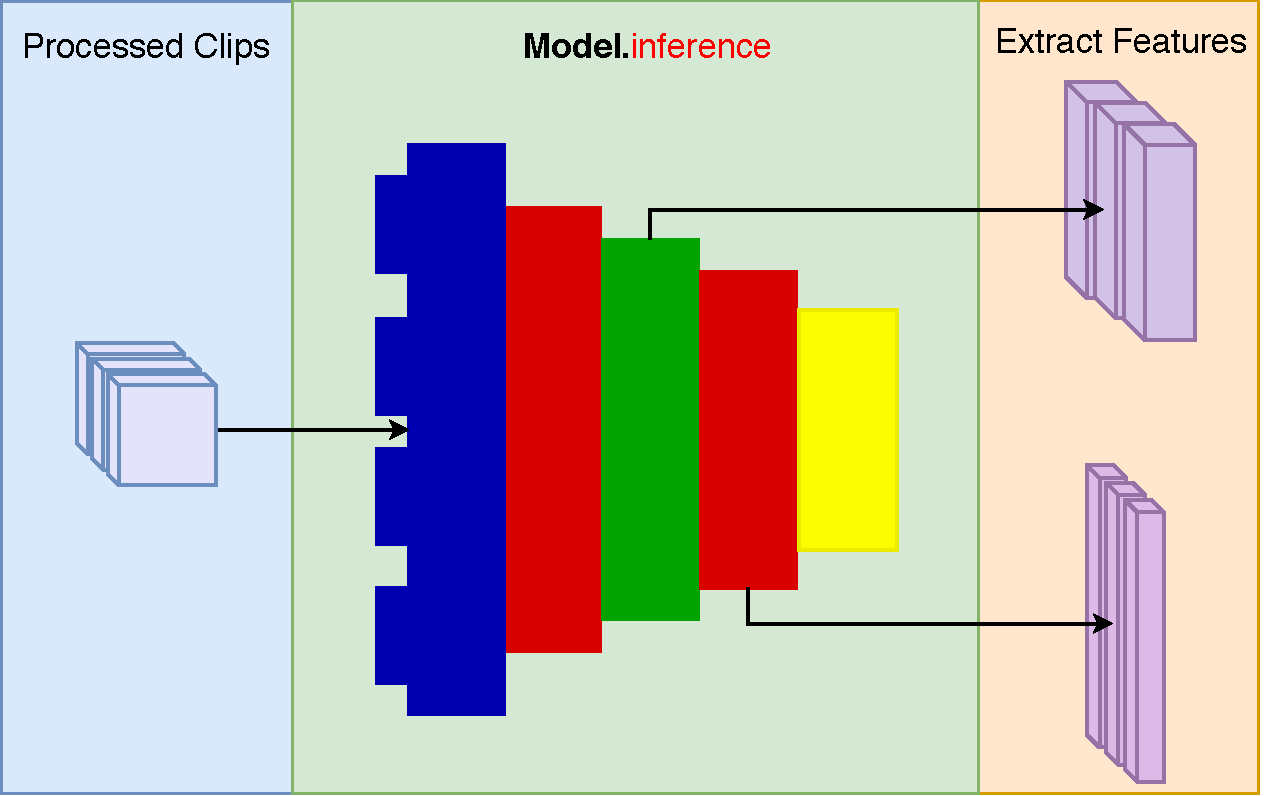
\includegraphics[width=0.7\columnwidth]{images/extract_features_h.pdf}
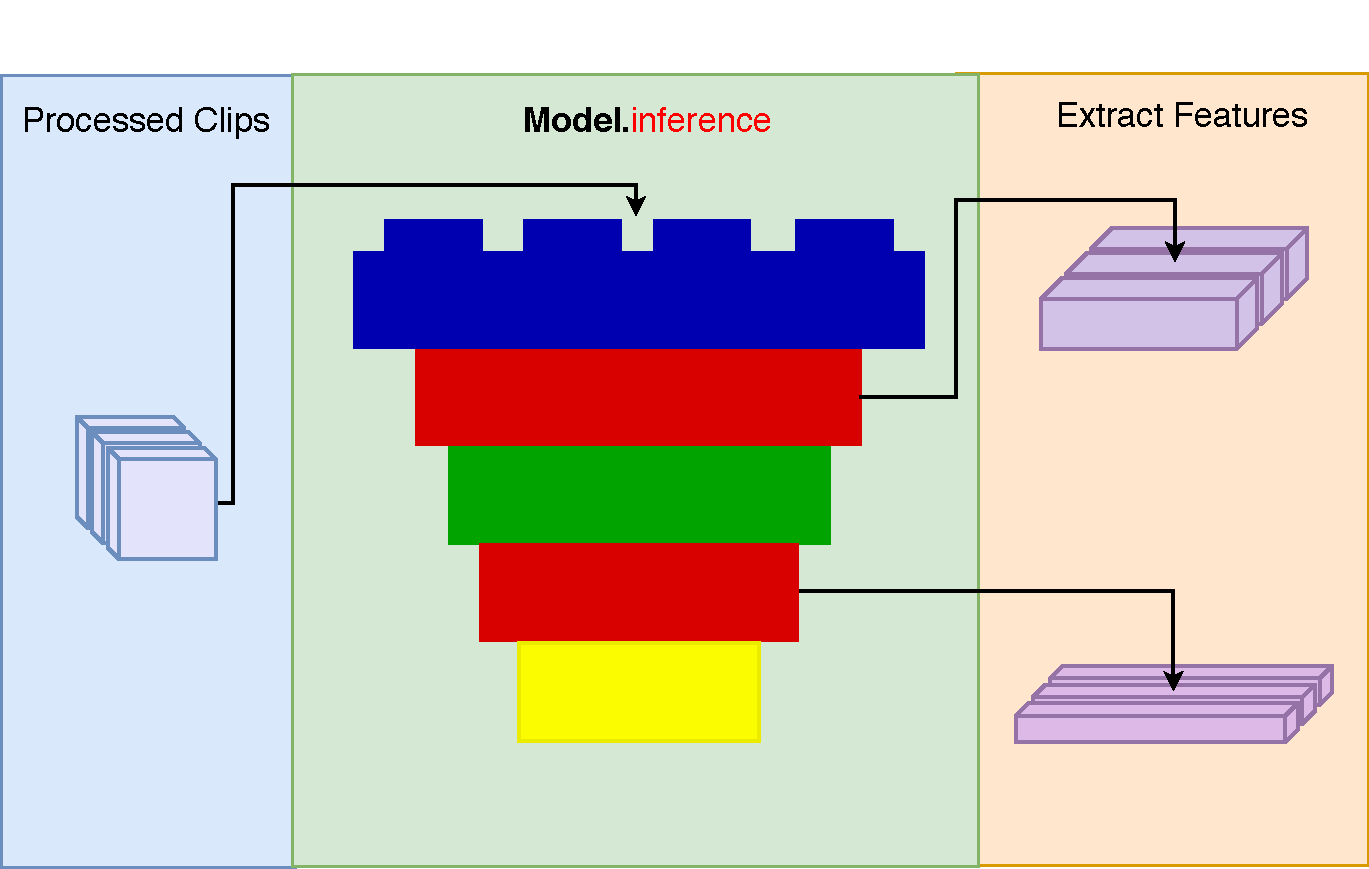
\includegraphics[width=0.7\columnwidth]{images/extract_features.pdf}
\caption{}
\label{fig:extract_features}
\end{figure}

\acro~offers a \textbf{Metrics Submodule} for testing and logging the activity recognition performance of a model as well as extracting features from a model.
This \textbf{Metrics Submodule} is incorporated in the testing pipeline as a class which gets instantiated in \textcolor{blue}{test.py}.
During testing, the output prediction, correct label, and name of each video which is loaded and passed through the model gets stored in this object during every iteration.
These performance metrics and other temporary data gets stored in an hdf5 file format and then deleted at the end of each testing session.
Hdf5 files are used for storing large amounts of temporary data due to their quick reading and writing capabilities.
Just before getting deleted, all relevent testing outputs are saved as numpy files.
Additionally, during testing, the chosen metric and any other specified varaible will be logged automatically using tensorboard.

Available performance metrics include average pooling, last frame prediction, and training a linear SVM classifier.
Average pooling is a common technique which uses the softmax predictions of a model's outputs and averages them across all frames of an input video.
From these predictions, the maximum value is used as the overall class prediction for that video.
The outputs of models can vary in shape so we standardize them to be in the form of [\texttt{\textcolor{ForestGreen}{batch\_size}}, \texttt{\textcolor{ForestGreen}{sequence\_length}}, \texttt{\textcolor{ForestGreen}{number\_of\_classes}}].
The \texttt{\textcolor{ForestGreen}{batch\_size}} parameter slightly changes meaning depending on the model being used.
For example for C3D, multiple clips can be loaded for a single video, the average can then be taken across all of these clips while the temporal dimensionality gets reduced from 16 frames to 1, removing the need for any average pooling or last frame prediction.
On the other hand, TSN would take multiple videos and refer to each as a single clip, thus the batch of different videos would each be logged separately.
\acro~is robust enough to handle both such cases.
Last frame classification is referenced originally in the ConvNet + LSTM model~\cite{}.
This technique calculates the argmax of solely the last frame of the input clip.
In addition to these metrics which directly classify the output of a model, \acro~also provides the option of training a linear SVM classifier based off of features extracted from any user specified layer within the model.
A linear SVM was used to classify video in the UCF101 dataset in C3D~\cite{}

Features can be extracted for a multitude of reasons other than just to train a linear SVM.
This quality allows \acro~to accomplish more than just activity recognition.
Any of the state-of-the-art models that have been implemented, or even any custom model, can be used for feature extraction.
With any dataset that has been converted to the proper tfrecords format, the correct input arguments allow the user to extract features from any layer in any available model.
Due to the large size that features can become over modern datasets with thousands and even millions of videos, it is crucial to be able to read and write them to memory quickly which is why we use an hdf5 file format for writing this data.




\section{Benchmarks}
\label{sec:benchmarks}

\begin{table}[tp!]
\begin{center}
\caption{Mean recognition accuracies are shown for various SOTA action recognition models across split 1 of HMDB51 and UCF101.
Values marked with a (*) indicate that  
Accuracies are reported for each baseline model and preprocessing technique combination.}
\label{tab:model_results}
\begin{tabular}{c|c|c|c||c|c}
\hline
\multirow{2}{*}{Base Model} & \multirow{2}{*}{Pretraining} & \multicolumn{2}{c||}{HMDB51} & \multicolumn{2}{c}{UCF101} \\\cline{3-6}
& & Our Acc & Author Acc & Our Acc & Author Acc \\
\hline
C3D & Sports-1M & --.-- & 50.30 * & --.-- & 82.30 * \\
\hline
I3D & Kinetics & --.-- & 74.30 * & --.-- & 95.1 * \\
\hline
TSN & ImageNet & --.-- & 54.40 & --.-- & 85.50 \\
\hline
ResNet50+LSTM & ImageNet & --.-- & 43.90 & --.-- & 84.30 \\
\hline
\end{tabular}
\end{center}
\end{table}


\section{Future Endeavors}
\label{sec:future}

\clearpage

\bibliographystyle{splncs}
\bibliography{egbib}

\end{document}

\grid
\grid
\grid
\grid
\grid
